\documentclass[12pt]{article}
\usepackage{amsmath,amsfonts, epsfig}
\usepackage{booktabs} % for better table formatting
\usepackage[authoryear]{natbib}
\usepackage{array}
\usepackage{multirow}
\usepackage{graphicx}
\usepackage{fancyhdr}
\usepackage{bm}
\pagestyle{fancy}
\lfoot{\texttt{ematm0067.github.io} / \texttt{ematm0044.github.io}}
\lhead{Introduction to AI - 02.5\_classifier - Conor}
\rhead{\thepage}
\cfoot{}

\usepackage{tikz}
\usetikzlibrary{positioning}

\usepackage{ifthen}
\newboolean{nopics}
\setboolean{nopics}{true}


\begin{document}

\section*{A linear classifier.} 

This section won't actually do anything that is different from the
logistic regression we described in the previous section; instead it
presents the same mathematics from a slightly different
perspective. In the logistic regression example we started with a
one-dimensional example, here we will look at another example, but
this time a higher dimensional one, based on data from Irish elections.

Elections in Ireland use an elegant voting system called Single
Transferable Vote that allows for constituency-based proportional
voting. There are multi-seat constituencies and votes transfer as
candidates are elected or eliminated, so it is a simplification to
reduce the votes to the proportion for each party. However, for our
purposes here this is what we have done. Based on the 2020
election\footnote{data.gov.ie/dataset/candidate-details-for-general-election-2020}
this figure show the fraction of `first preference' vote for two of
the main parties, Fianna F\'{a}il and Fine Gael, for all 39 constituencies.
\begin{center}
  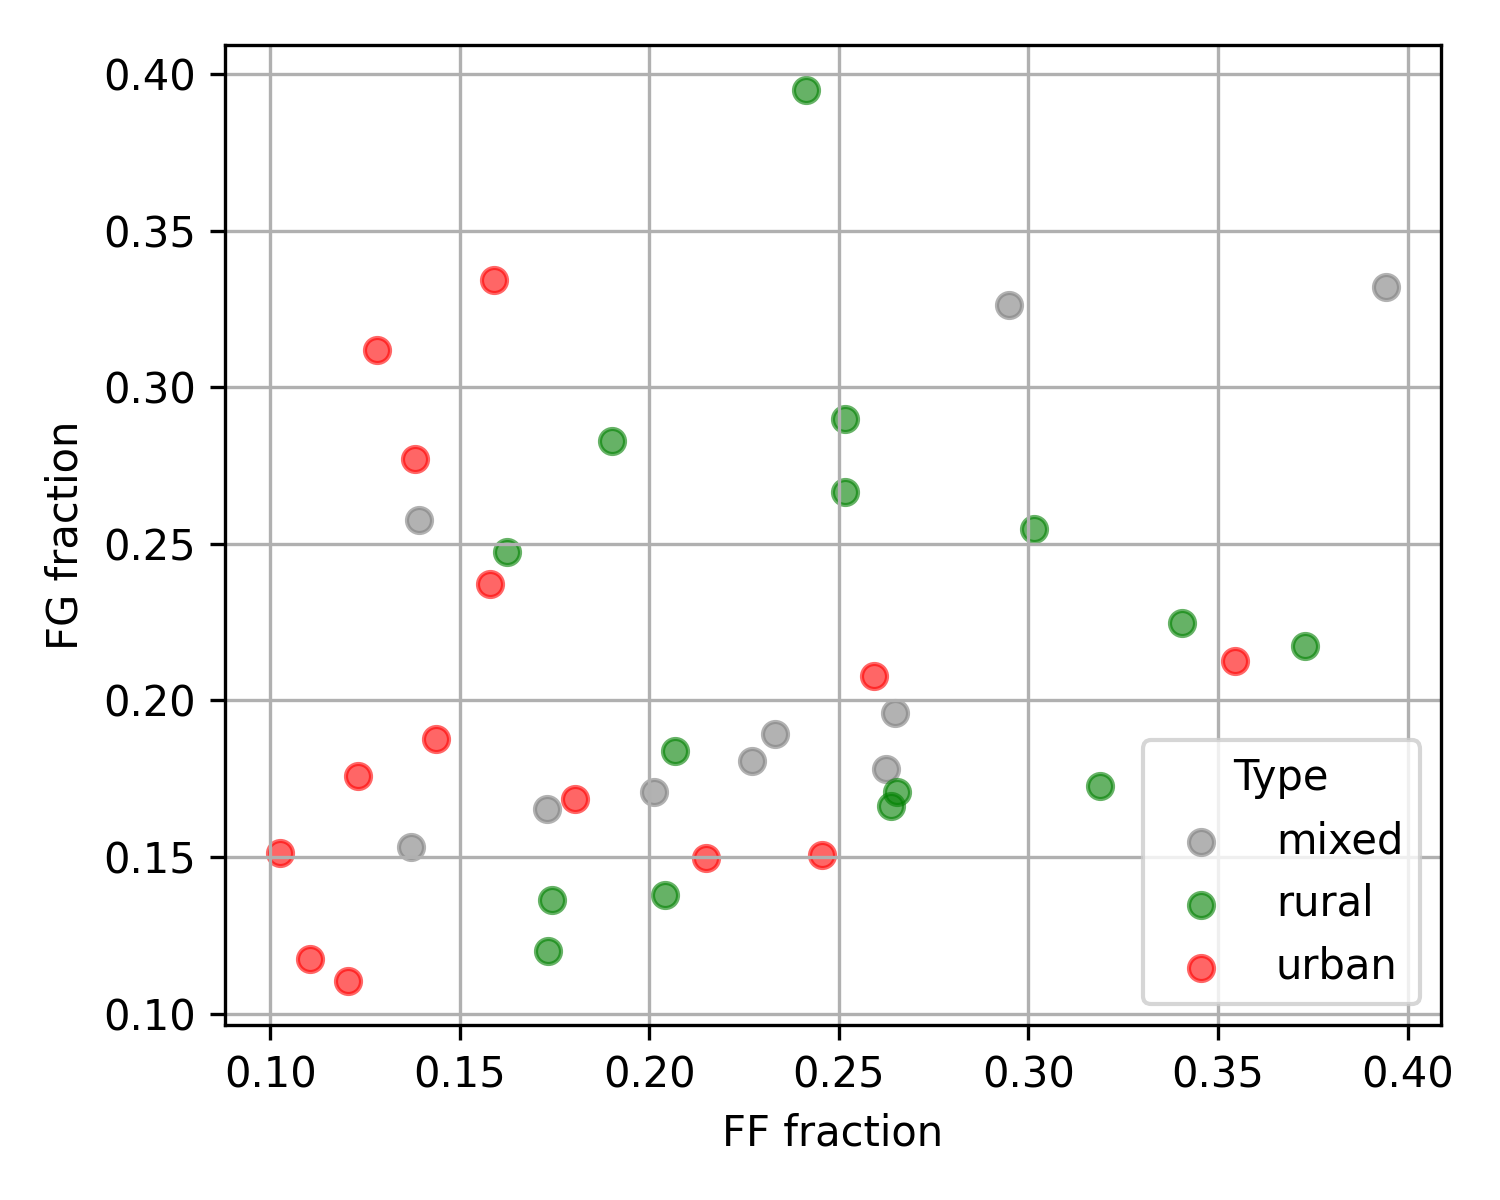
\includegraphics[]{02.5_ffVfg.png}
\end{center}
The constituencies have been labelled `urban', `mixed' and `rural' and
this has been marked by colour. Don't take these labels too seriously;
I guess it based on my own knowledge.

It is clear there is a relationship between the voting pattern and
settlement type with rural area more likely to vote for these two
parties. There are exceptions, in voting local issues often change the
result; the rural constituency Galway-Roscommon, for example, has
three TDs\footnote{Teachta D\'{a}l\'{a}, the title given to a
representative in Ireland}, one Sinn F\'{e}in, one who was in Fine
Gael who left in protest following the closure of a local hospital and
another who is an activist opposed to restrictions on the cutting of
turf, a significant issue in an area with large amounts of
bog. Similarly, the urban constituency with the largest Fianna
F\'{a}il vote is Cork South-Central; this is the constituency of
Miche\'{a}l Martin, who is leader of Fianna F\'{a}il, in the event he
went on to become Taoiseach\footnote{the equivalent of Premier or Prime
Minister} from 2020 to 2022.

Lets just concentrate on the urban and rural consistituencies and
imagine we want to guess the settlement type of an unknown
constituency based on the Fi\'{a}nna Fail and Fine Gael votes. The
obvious approach to that is to mark areas on the vote-fraction plane
corresponding to rural and urban constituencies and, in a linear model
that means dividing the plane using a straight line. In fact, this is
the same as the logistic regression tasks. In logistic regression we
modelled the probability using a logistic function:
\begin{equation}
  p(\text{rural})=\sigma(\beta_0+\beta_1x_1+\beta_2x_2)
\end{equation}
where, in our current context, $x_1$ is the fraction voting Fianna
F\'{a}il and $x_2$ the fraction voting Fine Gael. We found values for
the $\beta$s by optimising a loss function, the log-likelihood. With
these parameters we can then estimate a probability that any point is
`rural'; for a binary classified we can dump this nicety and just
predict that a constituency is rural if $p(\text{rural})\ge 0.5$. In
fact, $\sigma(0)=0.5$ so the decision boundary where
$\hat{p}(\text{rural})=0.5$ corresponds to
\begin{equation}
  \beta_0+\beta_1x_1+\beta_2x_2=0
\end{equation}
or, put another way, the line
\begin{equation}
  x_2=-\frac{\beta_1}{\beta_2}x_1-\frac{\beta_0}{\beta_2}
\end{equation}
Points to the above and to the right of this line have a greater than
0.5 estimated chance of being rural, those below and to the right,
less than 0.5.

We can plot that line
\begin{center}
  \includegraphics[]{02.5_ffVfg_linear.png}
\end{center}
We can see it has done ok, it isn't perfect, but then no line is going
to be. We can look at the assigned probability using a heatmap
\begin{center}
  \includegraphics[]{02.5_ffVfg_heatmap.png}
\end{center}
Clearly, it is has fitted the points as best as it can using a linear
classifier and this gives a useful model of settlement type, but a
linear model, perhaps unsurprisingly, has failed to account for Cork
South-Central, assigning it a high probability of being rural. We can
also see that the line is nearly vertical; the Fine Gael vote does not
seem to be playing a significant role in distinguishing rural and
urban. There is a complex history in this, Fianna F\'{a}il is a broad
party which lost a lot of support in the tumult surrounding the Great
Recession it lost support, particularly to Sinn F\'{e}in in urban
areas; however, Sinn F\'{e}in also has rural support so including it
isn't much better
\begin{center}
  \includegraphics[]{02.5_ffVsf.png}
\end{center}
There are lots of other parties we could consider, the left-wing and
social democratic parties like The Labour Party, The Green Party,
People Before Profits and The Social Democrats tend to do better in
cities. However, I don't want to get too distracted so lets stop. The data are on the github though if you want
to look, for example, if you want to do a classifier in higher
dimensions where the line will be replaced by a plane or hyperplane.

Another topic we won't consider here is the objective function, we
took the log-likelihood loss from logistic regression, but there are
others used for this problem. These approaches, some of which also
apply to regression, aim to \textsl{regularize}, that is, come up with
a fit that is less influenced by outliers and more likely to work on
unseen data; these leads to topics like \textsl{ridge regression},
\textsl{lasso regularizers} and \textsl{support vector machines}.
Regularization is, in general, something we will
consider more in the future. In the next section though, we will look
at the perceptron, which at first seems like a weird way to reformulate
linear classification but turns out to be useful.

\section*{Summary}
This is a straight-forward section in that it doesn't really introduce any new mathematics, all it does is replace the logistic regressor
\begin{equation}
  \hat{p}=\sigma(\beta_0+\bm{\beta}\cdot\mathbf{x})
\end{equation}
with the classification boundary corresponding to $\hat{p}=0$:
\begin{equation}
  \beta_0+\bm{\beta}\cdot\mathbf{x}=0
\end{equation}

\end{document}

